\documentclass{article}
\usepackage{ctex}
\usepackage{amsmath}
\usepackage{hyperref}
\usepackage{fancyhdr}
\usepackage{fontspec}
\usepackage{graphicx}
\usepackage{subfigure}
\setmainfont[Mapping=tex-text]{KaiTi}

\topmargin=-0.45in
\evensidemargin=0in
\oddsidemargin=0in
\textwidth=6.5in
\textheight=9.0in
\headsep=0.25in
\linespread{1.1}



%配置区
\newcommand{\courseName}{模式识别}
\newcommand{\homeworkId}{\#4} %作业编号
\newcommand{\homeworkTitle}{作业\homeworkId}
\newcommand{\studentId}{201928014629008}%学号
\newcommand{\studentName}{牛李金梁}%姓名

\newcommand{\question}[1]{\section*{Question #1}}
\renewcommand{\part}[1]{\subsection*{(#1)}}

\pagestyle{fancy}
\lhead{\studentName}
\rhead{\courseName\homeworkTitle}
\cfoot{\thepage}

\title{
    \vspace{2in}
    \textmd{\textbf{\courseName}:\homeworkTitle}\\
    \vspace{0.1in}
    \large{\studentId}\\
    \large{\studentName}\\
    \vspace{3in}
}

\begin{document}


\maketitle
\date{}
\pagebreak

\section*{第一部分:计算与证明}

\question{1}
\part{a}
记第$k$个样本${\pmb{x}^k} = {\left[ {1,x_1^k,x_2^k, \cdots ,x_d^k} \right]^T}$。
设隐含层有$n$个神经元,
输入层到隐含层的连接权重为$\left( {d + 1} \right) \times n$维的矩阵${W^H}$,
其中某个元素记为${w_{ih}}$;输出层有$c$个神经元,
隐含层到输出层的连接权重为$\left( n \right) \times c$维的矩阵${W^c}$,
其中某个元素记${w_{hj}}$。

在前馈过程中,隐含层$h$结点的输出为
$y_h^k = {f_1}\left( {net_h^k} \right) = f\left( {\sum\limits_i {{w_{ih}}x_i^k} } \right)$
,$f$为sigmoid函数;输出层$j$结点的输出为
$z_j^k = {f_2}\left( {net_j^k} \right) = f\left( {\sum\limits_h {{w_{hj}}y_h^k} } \right) = {f_2}\left( {\sum\limits_h {{w_{hj}}{f_1}\left( {\sum\limits_i {{w_{ih}}x_i^k} } \right)} } \right)$
,$f$为softmax函数。

误差函数为
\begin{align*}
	E{\left( w \right)^k} = J{\left( w \right)^k} 
	&= {1 \over 2}\sum\limits_j {{{\left( {t_j^k - z_j^k} \right)}^2}} \\
	&= {1 \over 2}\sum\limits_j {{{\left( {t_j^k - f\left( {net_j^k} \right)} \right)}^2}} \\
	&= {1 \over 2}\sum\limits_j {{{\left( {t_j^k - f\left( {\sum\limits_h {{w_{hj}}f\left( {net_h^k} \right)} } \right)} \right)}^2}} 
\end{align*}

隐含层到输出层的连接权重调节量:
\begin{align*}
	\Delta {w_{hj}} 
	&=  - \eta {{\partial E} \over {\partial {w_{hj}}}} 
	= - \eta \sum\limits_k {{{\partial E} \over {\partial net_j^k}}{{\partial net_j^k} \over {\partial {w_{hj}}}}}\\
	&= \eta \sum\limits_k {\left( {t_j^k - z_j^k} \right)f'\left( {net_j^k} \right)y_h^k} \\
	&= \eta \sum\limits_k {\delta _j^ky_h^k} 
\end{align*}

其中,$\delta _j^k =  - 
{{\partial E} \over {\partial net_j^k}} = 
f'\left( {net_j^k} \right)\left( {t_j^k - z_j^k} \right)$,
$f$为softmax函数。softmax的导数为雅可比矩阵,此处需要的
是矩阵主对角线上的元素。设softmax主对角线上的第$j$个元素
是$S_j$,有${{S_j}'} = {S_j}\left( {1 - {S_j}} \right)$。

因此,$\Delta {w_{hj}} =
\eta \sum\limits_k {\left( {t_j^k - z_j^k} \right)
{S_j}\left( {1 - {S_j}} \right)y_h^k} $,其中,
${S_j} = {{\exp \left( {net_j^k} \right)} 
\over {\sum\limits_i {\exp \left( {net_i^k} \right)} }}$

输入层到隐含层的连接权重调节量:
\begin{align*}
	\Delta {w_{ih}} 
	=  - \eta {{\partial E} \over {\partial {w_{ih}}}} 
	&=  - \eta \sum\limits_{k,j} {{{\partial E} \over {\partial z_j^k}}{{\partial z_j^k} \over {\partial {w_{ih}}}}} \\
	&= \eta \sum\limits_{k,j} {\left( {t_j^k - z_j^k} \right){{\partial z_j^k} \over {\partial {w_{ih}}}}} \\
	&= \eta \sum\limits_{k,j} {\left( {t_j^k - z_j^k} \right){{\partial z_j^k} \over {\partial net_j^k}}} {{\partial net_j^k} \over {\partial {w_{ih}}}}\\
	&= \eta \sum\limits_{k,j} {\left( {t_j^k - z_j^k} \right)f'\left( {net_j^k} \right)} {{\partial net_j^k} \over {\partial y_h^k}}{{\partial y_h^k} \over {\partial {w_{ih}}}}\\
	&= \eta \sum\limits_{k,j} {\left( {t_j^k - z_j^k} \right)f'\left( {net_j^k} \right)} {w_{hj}}{{\partial y_h^k} \over {\partial {w_{ih}}}}\\
	&= \eta \sum\limits_{k,j} {\left( {t_j^k - z_j^k} \right)f'\left( {net_j^k} \right)} {w_{hj}}{{\partial y_h^k} \over {\partial net_h^k}}{{\partial net_h^k} \over {\partial {w_{ih}}}}\\
	&= \eta \sum\limits_{k,j} {\left( {t_j^k - z_j^k} \right)f'\left( {net_j^k} \right)} {w_{hj}}f'\left( {net_h^k} \right)x_i^k\\
	&= \eta \sum\limits_k {\delta _h^k} x_i^k
\end{align*}

其中,$\delta _h^k =  - {{\partial E} \over {\partial net_h^k}} = f'\left( {net_h^k} \right)\sum\limits_j {{w_{hj}}\delta _h^k} $,$\delta _j^k = f'\left( {net_j^k} \right)\left( {t_j^k - z_j^k} \right)$。

sigmoid函数的导数${{S_h}'} = {{S_h}\left( {1 - {S_h}} \right)}$,于是,$\Delta {w_{ih}} 
= \sum\limits_j {{w_{hj}}\delta _j^k} {S_h}\left( {1 - {S_h}} \right)x_i^k$,${S_h} = {1 \over {1 + \exp \left( { - net_h^k} \right)}}$

\part{b}
通过(a)中的推导可以看出,反向传播算法将各层间的连接权重分隔开,
使之相互独立,传播时输出层的误差沿着前馈网络的反方向
逐层更新层间的连接权重,从而避免了深层网络中复合函数链式求导中过长的链。
这一算法对简化神经网络优化过程有着重要的意义。

\question{2}
计算步骤:
\begin{itemize}
	\item[-] 初始化网络。通常使用随机初始化的方法。
	\item[-] 输入训练样本,每个样本为一个$d$维向量。
	\item[-] 计算映射层的权重向量和输入向量的距离。
		${d_j} = \sqrt {\sum\limits_{i = 1}^d {{{\left( {{x_i} - {w_{ij}}} \right)}^2}} } $。
	\item[-] 选择与权重向量距离最小的神经元作为胜出神经元${j^*}$,并给出其邻接
		神经元集合$h\left( {.,{j^*}} \right)$
	\item[-] 调整胜出神经元和其邻接神经元的权重,按下式更新:
	$$\Delta {w_{ij}} = \eta h\left( {j,{j^*}} \right)\left( {{x_i} - {w_{ij}}} \right)$$
	$${w_{ij}}\left( {t + 1} \right) = {w_{ij}}\left( t \right) + \Delta {w_{ij}}$$
	\item[-] 检查是否达到预设要求,是则结束算法,否则进行迭代。
\end{itemize}

算法流程图:
\begin{figure}[ht]
	\centering
	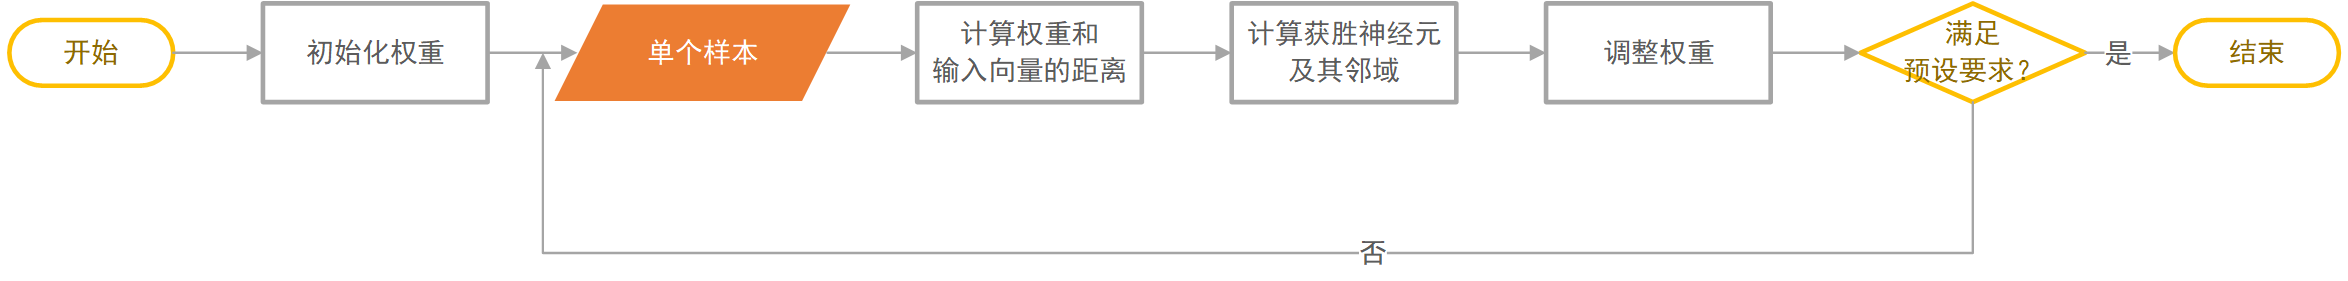
\includegraphics[width=1\textwidth]{Figure_2.png}
	\caption{自组织算法流程图}
	\label{figl}
\end{figure}

\question{3}
\part{1}

\begin{description}
	\item [\pmb{输入}] 图像大小:${\rm{400}} \times {\rm{400}}$
	\item [\pmb{第一卷积层}] 
	
	滤波器大小:${\rm{5}} \times {\rm{5}}$

	结点图像个数:$20$

	图像大小:${\rm{396}} \times {\rm{396}}$
	
	pooling后图像大小:${\rm{198}} \times {\rm{198}}$
	
	包含偏置的训练权重个数:${\rm{5}} \times {\rm{5}} \times {\rm{20 + 20 = 520}}$

	\item [\pmb{第二卷积层}] 
	滤波器大小:${\rm{3}} \times {\rm{3}} \times {\rm{20}}$

	结点图像个数:$30$

	滤波器总数:$30$

	图像大小:${\rm{196}} \times {\rm{196}}$
	
	pooling后图像大小:${\rm{98}} \times {\rm{98}}$
	
	包含偏置的训练权重个数:${\rm{20}} \times {\rm{3}} \times {\rm{3}} \times {\rm{30 + 30 = 5430}}$
	
	\item[\pmb{第三卷积层}]	
	滤波器大小:${\rm{3}} \times {\rm{3}} \times {\rm{30}}$

	结点图像个数:$20$

	滤波器总数:$20$
	
	图像大小:${\rm{96}} \times {\rm{96}}$
	
	pooling后图像大小:${\rm{48}} \times {\rm{48}}$
	
	包含偏置的训练权重个数:${\rm{30}} \times {\rm{3}} \times {\rm{3}} \times {\rm{20 + 20 = 5420}}$
	
	\item[\pmb{第四卷积层}]
	滤波器大小:${\rm{3}} \times {\rm{3}} \times {\rm{10}}$

	结点图像个数:$10$

	滤波器总数:$10$

	特征图尺度:${\rm{46}} \times {\rm{46}}$
	
	pooling后图像大小:${\rm{23}} \times {\rm{23}}$
	
	包含偏置的训练权重个数:${\rm{20}} \times {\rm{3}} \times {\rm{3}} \times {\rm{10 + 10 = 1810}}$

	\item[\pmb{全连接层}]
	输入图像大小: ${\rm{23}} \times {\rm{23}}$

	输入图像个数:$10$

	输出结点个数:$10$
	
	包含偏置的训练权重个数:${\rm{10}} \times {\rm{23}} \times {\rm{23}} \times {\rm{10 + 10 = 52910}}$
\end{description}
采用权值共享和局部连接的总权重个数为65290。
\\\\
\pmb{采用全连接网络}:

输入层到第一隐层:${\rm{400}} \times {\rm{400}} \times {\rm{396}} \times {\rm{396}} \times {\rm{20 + 396}} \times {\rm{396}} \times {\rm{20 = 501814336320}}$

第一隐层到第二隐层:${\rm{198}} \times {\rm{198}} \times {\rm{20}} \times {\rm{196}} \times {\rm{196}} \times {\rm{30 + 196}} \times {\rm{196}} \times {\rm{30 = 903637670880}}$

第二隐层到第三隐层:${\rm{98}} \times {\rm{98}} \times {\rm{30}} \times {\rm{96}} \times {\rm{96}} \times {\rm{20 + 96}} \times {\rm{96}} \times {\rm{20 = 53106462720}}$

第三隐层到第四隐层:${\rm{48}} \times {\rm{48}} \times {\rm{20}} \times {\rm{46}} \times {\rm{46}} \times {\rm{10 + 46}} \times {\rm{46}} \times {\rm{10 = 975073960}}$

第四隐层到输出层:${\rm{23}} \times {\rm{23}} \times {\rm{10}} \times {\rm{10 + 10}} \times {\rm{10 = 53000}}$

总权重个数约为${\rm{1}}{\rm{.459}} \times {\rm{1}}{{\rm{0}}^{{\rm{12}}}}$。
\\\\
\pmb{不采用权值共享}:

输入层到第一隐层:${\rm{5}} \times {\rm{5}} \times {\rm{396}} \times {\rm{396}} \times {\rm{20 + 396}} \times {\rm{396}} \times {\rm{20 = 105304320}}$

第一隐层到第二隐层:${\rm{3}} \times {\rm{3}} \times {\rm{20}} \times {\rm{196}} \times {\rm{196}} \times {\rm{30 + 196}} \times {\rm{196}} \times {\rm{30 = 208598880}}$

第二隐层到第三隐层:${\rm{3}} \times {\rm{3}} \times {\rm{30}} \times {\rm{96}} \times {\rm{96}} \times {\rm{20 + 96}} \times {\rm{96}} \times {\rm{20 = 49950720}}$

第三隐层到第四隐层:${\rm{3}} \times {\rm{3}} \times {\rm{20}} \times {\rm{46}} \times {\rm{46}} \times {\rm{10 + 46}} \times {\rm{46}} \times {\rm{10 = 3829960}}$

第四隐层到输出层:${\rm{23}} \times {\rm{23}} \times {\rm{10}} \times {\rm{10 + 10}} \times {\rm{10 = 53000}}$

总权重个数约为${\rm{3}}{\rm{.67}} \times {\rm{1}}{{\rm{0}}^{\rm{8}}}$。
\\\\
与二者相比,采用权值共享和局部连接的总权重个数基本可以忽略。

\part{2}
max pooling的前向传播是舍去其他元素,把区域内最大的值传给后一层。
反向传播则把梯度直接传给前一层该区域的某一个像素,
而其他像素为0。
确定这个像素需要记录下pooling时取的是哪个像素,
即最大值所在位置。

\part{3}
能改变网络结构的因素:
\begin{itemize}
	\item[-] 改变网络层数
	\item[-] 采用不同大小的滤波器
	\item[-] 激励函数的选择
	\item[-] 池化操作的选择
	\item[-] 能量函数的选择
\end{itemize}

\section*{第二部分:计算机编程}
环境为python3.7

依赖库:numpy、matplotlib

运行方式:直接在cmd中执行相应py文件

\question{1}
对于3层前向神经网络并使用反向传播进行训练,要确定以下参数:
\begin{itemize}
	\item[-] 批大小
	\item[-] 隐层结点个数
	\item[-] 梯度更新步长
	\item[-] 训练次数
\end{itemize}
还要根据已知参数确定输入层结点个数(样本维度),输出层类别个数。

具体训练中,先随机初始化层间权重,接着进行多次迭代。将数据分批送入
网络前向传播,并根据误差函数(平方误差)计算误差,然后将误差反向
传播来修正层间权值。经过迭代,误差越来越小,直到迭代次数满足预设的训练次数,
则根据预测判断正确率。

\question{2}
\part{a}
隐含层结点个数从1到10逐步增加,计算误差和训练集准确率,得到下面的图。
\begin{figure}[ht]
	\centering
	\subfigure{
		\begin{minipage}[t]{0.45\linewidth}
			\centering
			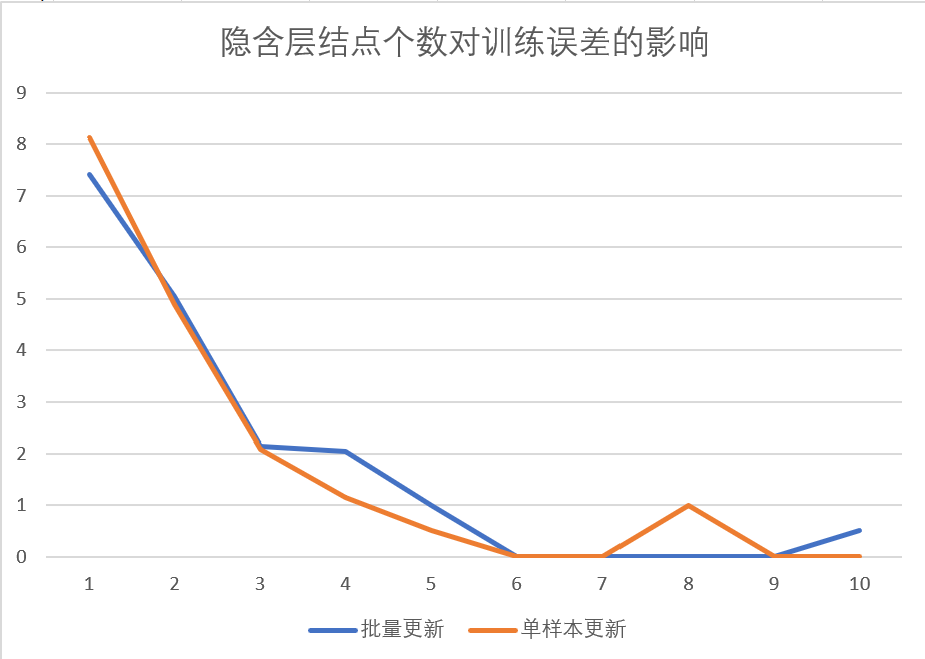
\includegraphics[width=3in]{a_1.png}
		\end{minipage}
	}
	\subfigure{
		\begin{minipage}[t]{0.45\linewidth}
			\centering
			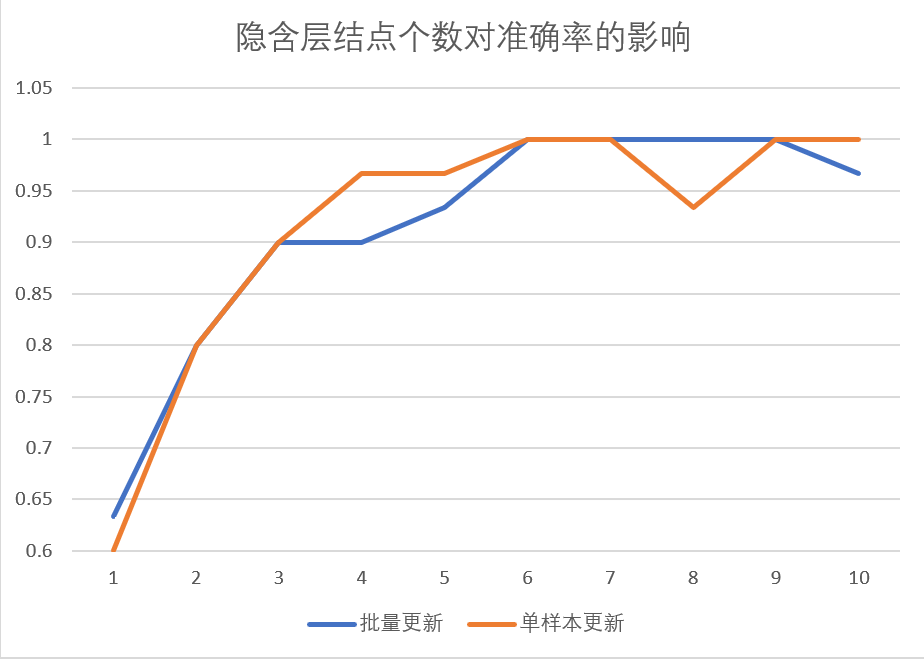
\includegraphics[width=3in]{a_2.png}
		\end{minipage}
	}
	\centering
	\caption{隐含层结点个数对训练精度的影响}
	\label{figl}
\end{figure}

从图可知,随着隐含层结点数目的增加,训练误差整体趋势是减小,分类准确率整体趋势是增加。
但也可以看出,结点数并不需要无限制的增加,只需要采用适当的结点数,便可以有效地进行训练了。

\part{b}
设定隐含层结点数为8,梯度更新步长从0.002到0.2以0.002的步长变化,得到下面的图。
\begin{figure}[ht]
	\centering
	\subfigure{
		\begin{minipage}[t]{0.45\linewidth}
			\centering
			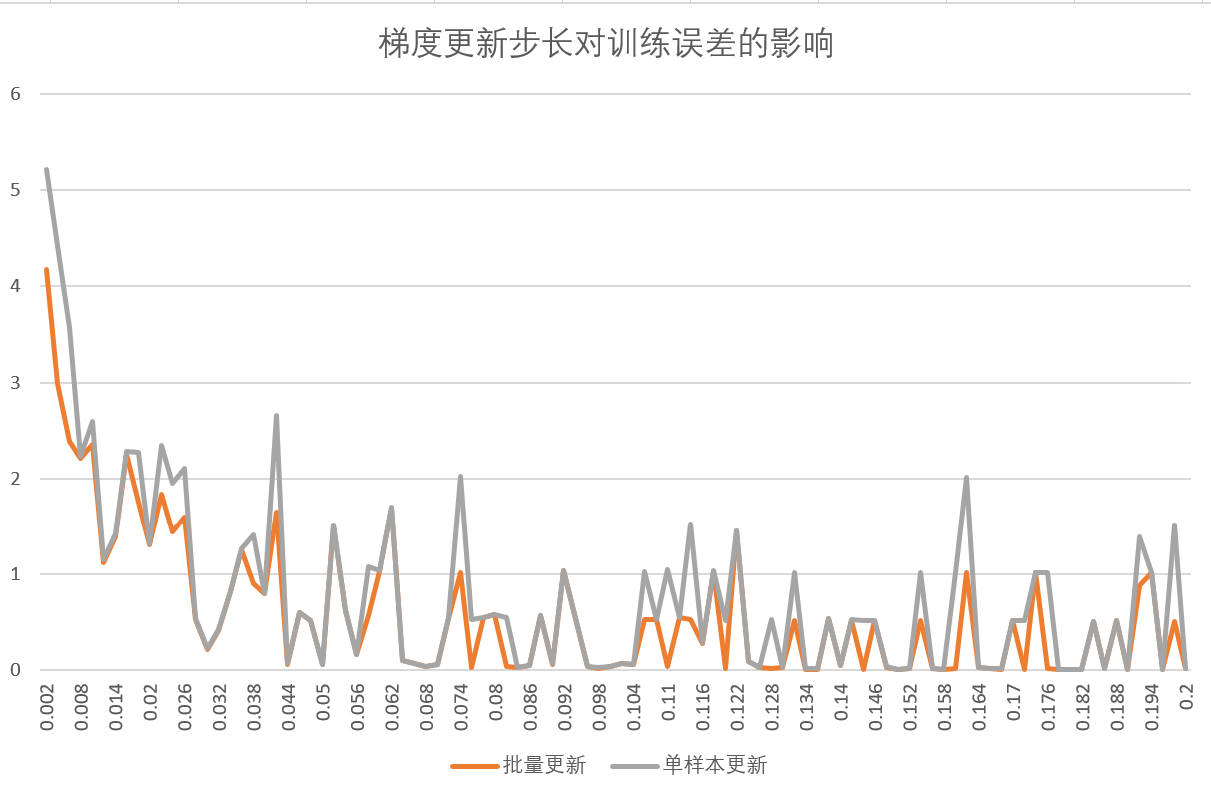
\includegraphics[width=3in]{b_1.png}
		\end{minipage}
	}
	\subfigure{
		\begin{minipage}[t]{0.45\linewidth}
			\centering
			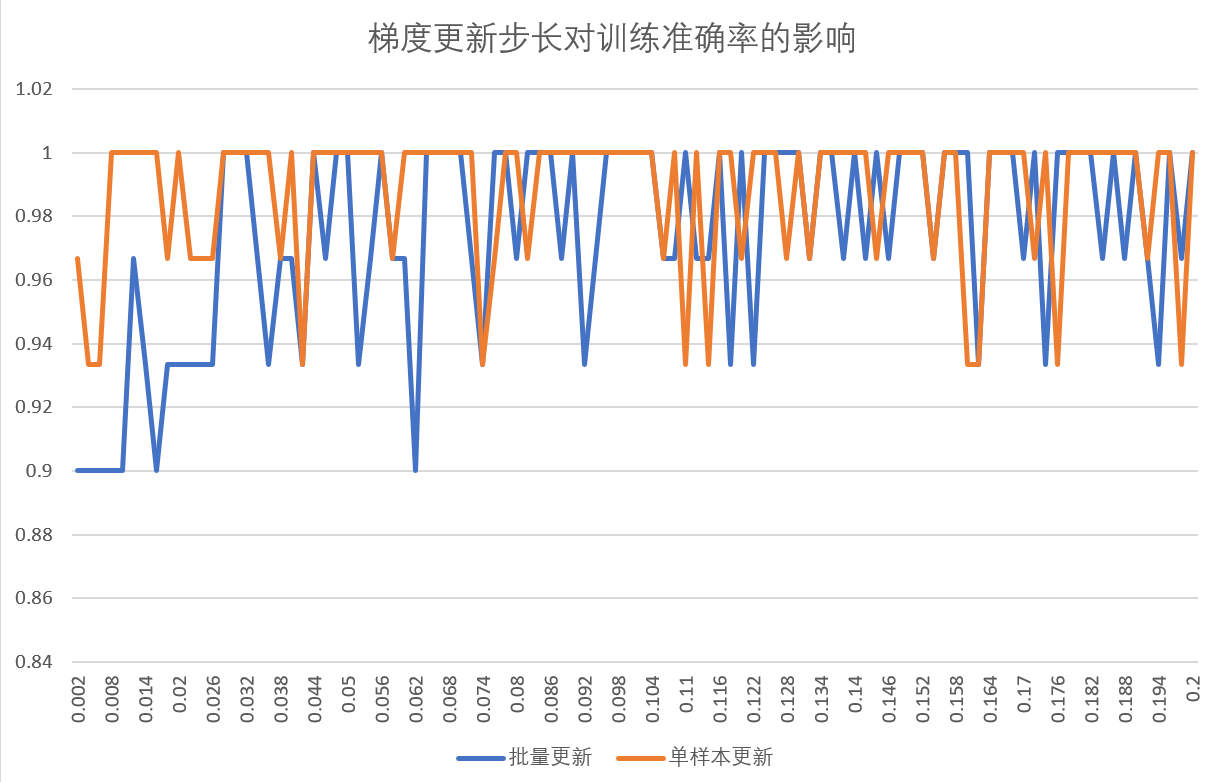
\includegraphics[width=3in]{b_2.png}
		\end{minipage}
	}
	\centering
	\caption{梯度更新步长对训练的影响}
	\label{figl}
\end{figure}

从图中可以看出,随着更新步长的增加,训练误差呈先减小后增加的态势,
训练准确率也呈先提高后减小的态势。

出现这种情况是因为以较小的更新步长进行训练时,在有限迭代次数内仍未
收敛,所以此时的误差较高准确率较低。而对于较大的更新步长,由于更新步长过大,
所得的解一直在最优值附近徘徊却无法到达,因此误差和准确率出现了震荡。

因此,网络训练中应采取合适的更新步长,过小则收敛慢,过大则效果不好。

\part{3}
本实验将epoch设为1000,采用批量更新的方法,batch size设为10,即总共进行
3000次迭代,隐含层结点数为8,学习率为0.1,结果如下图所示。
\begin{figure}[ht]
	\centering
	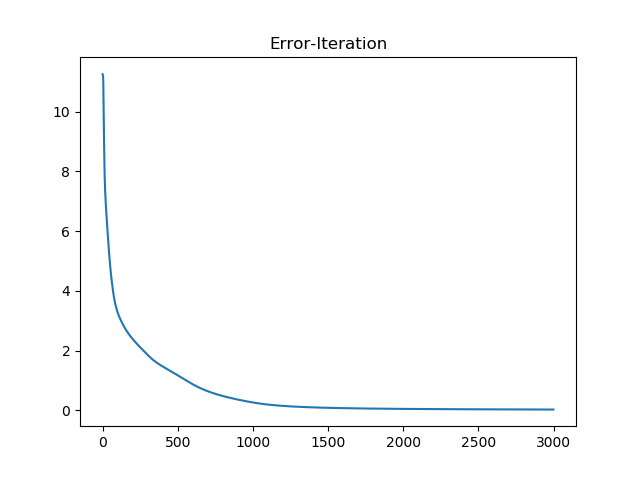
\includegraphics[width=0.5\textwidth]{c.png}
	\caption{目标函数随迭代次数增加的变化}
	\label{figl}
\end{figure}
从图中可以看出,本程序有良好的收敛特性。
\end{document}